\chapter{Modeling}
All models of the robotic manipulator were Matlab based. The first models were made simply as tests for the kinematics calculations. Given a set of angles the manipulator was drawn as a line between each of the joint positions. Each of these positions is calculated using the A matrices calculated for the joints as described in the Kinematics' section. So the first joint is calculated by the last column of A. Location of the second joint is located at $A_1A_2$'s fourth column and so on. The origin, (0,0,0) is selected as the origin of the manipulator, the start of the first joint. The result of this is shown in Figure \ref{fig:matlab}. With this setup it was possible to test the actions of the manipulator based on different functions.

\begin{figure}
\centering
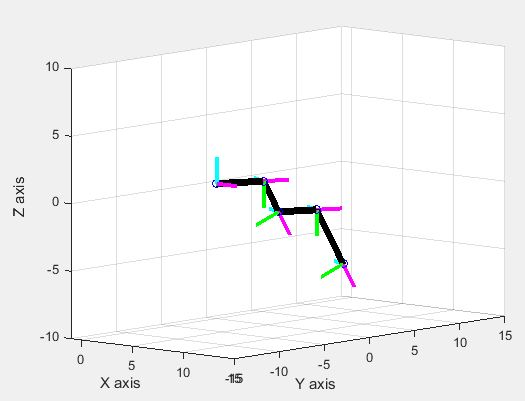
\includegraphics[width=0.5\textwidth]{matlabarm}
\caption{Arm graphed onto 3D image in Matlab.}
\label{fig:matlab}
\end{figure}

The inverse kinematics was tested using this model before testing on the real manipulator. The inverse kinematics equations along with the joint limits were programmed into a matlab function. The program could draw the resulting arm configuration for any desired end effector position in the workspace. For cases was not solvable the arm simply did not move, this was determined using the inverse kinematics feasibility test described in Chapter 3. The physical constraints were also programmed into the code to stop the arm for traveling outside of the physical angle limitations. Testing this code confirmed that the workspace of the manipulator is convex. This means that from one existing point in the workspace to other point in the workspace then the line between them is also in the workspace. This fact was use to create a trajectory from a starting position to a desired end position by calculating the linear path between them.

The next model was made to test the path planning code. In matlab obstacles were drawn on the 3D graph with the centers at the inputted obstacle value. The path planning algorithm then computed the path for the manipulator which was drawn through each configuration in the path. This model showed the algorithm to be able to consistently make it to the desired obstacle location with a smooth trajectory. The matlab simulation did not include any modeling of the gripper simply showing the path to the obstacle. An image of this simulation is shown in Figure \ref{fig:pathmatlab}.

\begin{figure}[h]
\centering
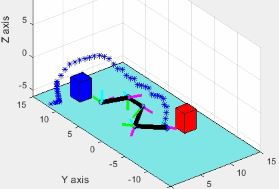
\includegraphics[width=0.5\textwidth]{pathmatlab}
\caption{Path planning simulation in matlab.}
\label{fig:pathmatlab}
\end{figure}

A more realistic model of the manipulator was created in the Virtual Robo Experimentation Platform (V-REP). This software includes physics engines which could more accurately simulated the manipulator at he goal objects reactions. First the servo and brackets 3D models were downloaded and the arm was assembled in Solidworks to create an accurate model of the manipulator. The 3D model was imported into V-REP and each servo set as a joint. Obstacles were created a similar size, shape, and weight as the real obstacles 3D printed for this project. The same matlab code was used to control the joint angles in V-REP. The simulation was then run and used to pick up objects. 

The V-REP simulation was not as reliable as the matlab simulation and a few code changes needed to be made to avoid the open gripper hitting the obstacles. There were also some problems with the objects flying out of the gripper. This seemed to  be a result of the physics engine and after a few adjustments to the object materials the simulation successfully picked up the object. An image of this simulation is shown in Figure \ref{fig:pathvrep}. The results of this simulation made it seem as though the path planning algorithm was likely to work with the real manipulator but would likely need some tuning to successfully grab objects. 

\begin{figure}
\centering
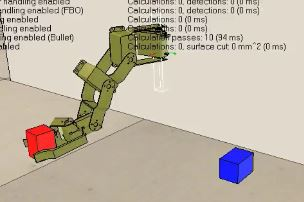
\includegraphics[width=0.5\textwidth]{pathplan}
\caption{Path planning model in V-REP.}
\label{fig:pathvrep}
\end{figure}